\section{Visualization's Tools}

Visualization tools are supposed to supplement the domain expertise and deliver a big image so that users are able to frame critical questions and later propose heuristic and insightful answers to these questions \cite{kung2015visualization}. Traditional tools like Excel can not or at least struggle to perform visual analytics on big data involving millions of records so new visualization tools or enhancements in existing tools were on demands to handle the complexity of big data \cite{nair2016interactive}. There are dozens, if not hundreds of tools available to create a visualization of large data sets. Most of them are basic and have a lot of overlapping tools. One way to categorize tools is whether they are drag and drop types or they require coding for creating a visualization. Most of the proprietary visualizations tools are from the drag and drop type, which requires no coding skills. Although it is easy to learn and create visualizations in minutes the drawback is that out-of-box visualizations are not possible \cite{nair2016interactive}. In this section, the focus is on the standouts that either have more capability for the types of visualizations they can create and the amount of freedom in customization they can offer or are significantly easier to use than the other options out there. 

\subsection{Tableau}

Tableau is a leading data visualization tool used for data analysis and business intelligence. It is capable of delivering interactive visualizations in no time with its drag and drop nature. Gartner’s Magic Quadrant classified Tableau as a leader for analytics and business intelligence \cite{parenteau2016magic}. Tableau is a user-friendly tool and was built for a diverse amount of teams. It is an easy-to-use tool that requires no programming skills and it provides results in a wide variety of formats. It can be connected to the data stored in excel, CSV, and text files and recognize fields and formats. Moreover, it provides integration with all the major advanced databases, including Teradata, SAP, My SQL, Amazon AWS, and Hadoop. Below are some of the main advantages and disadvantages of using Tableau to visualize big data. To meet the need of diverse users, Tableau software provides selections that include Tableau Desktop, Tableau Server, and Tableau Mobile to choose from. As Tableau Desktop is preferred by individuals and small organizations, Tableau Server is more convenient for big organizations with many users.

On the other hand, it is a very expensive product to scale across huge organizations. Moreover, it provides a very basic prepossessing so in most cases data needs to be exported in perfect tables. Finally, no out-of-the-box visualizations can be provided and users have to stick to the offered ones.


\begin{figure}[H]
\centering
\captionsetup{justification=centering}
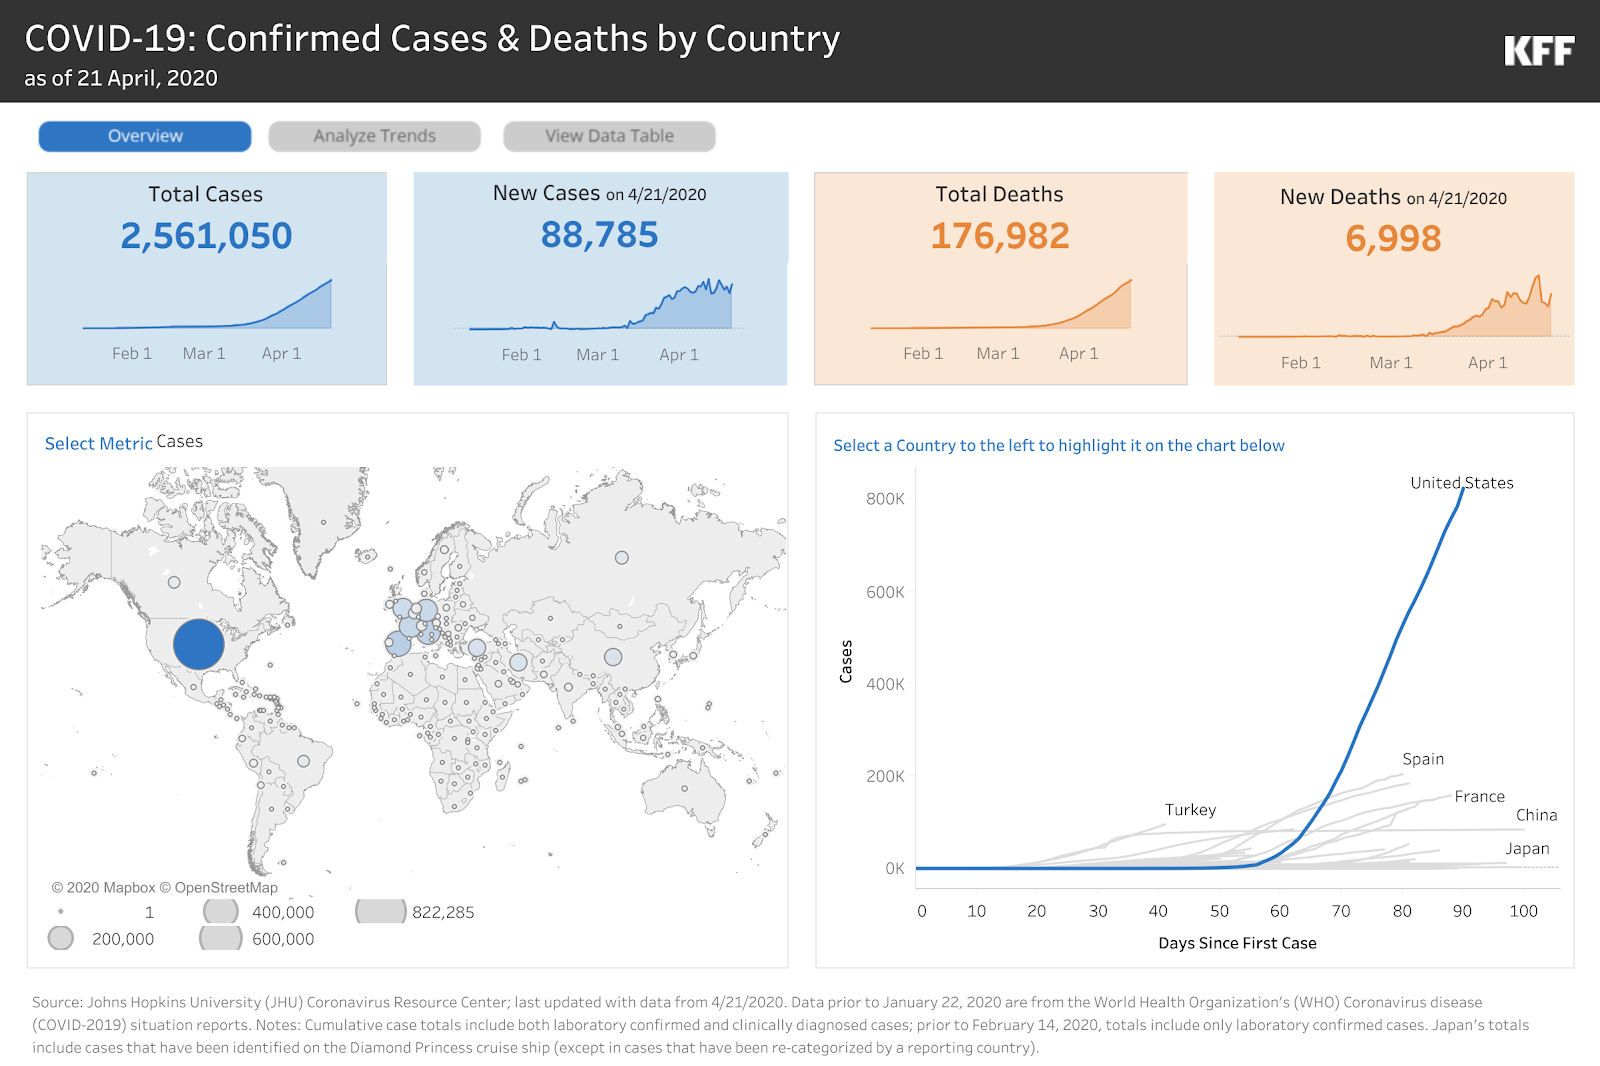
\includegraphics[width=0.9\textwidth]{Report-latex/tex_files/pics/tableau.png}
\caption{Tableau dashboard example from (JHU) Coronavirus resource center}
\end{figure}



\subsection{D3.js}

D3 is a free open source tool that makes any visualization possible and in fact, many visualization libraries where JavaScript is the coding language are built on top of D3. D3 outperforms all other JavaScript-based tools as it offers versatile functionalities like data manipulation and transformation and makes effective use of the power of new browser and web technologies \cite{nair2016interactive}. It can create very powerful and highly interactive visualizations. As it requires coding skills in JavaScript, CSS, and HTML any basic visualization needs to be coded from scratch. However, D3 has a big community and many built-in reusable functions, and samples of commonly used graphics are available. Basically, D3 can create any imaginable visualization and offers excellent interactivity within coding limits. 

Not supporting older browsers and the programming experience needed to even create simple visualizations are some of the disadvantages that would hold users from using D3. Usually, easier tools with fewer lines of codes would be used unless customization and performance are priorities especially with big data. 

\begin{figure}[H]
\centering
\captionsetup{justification=centering}
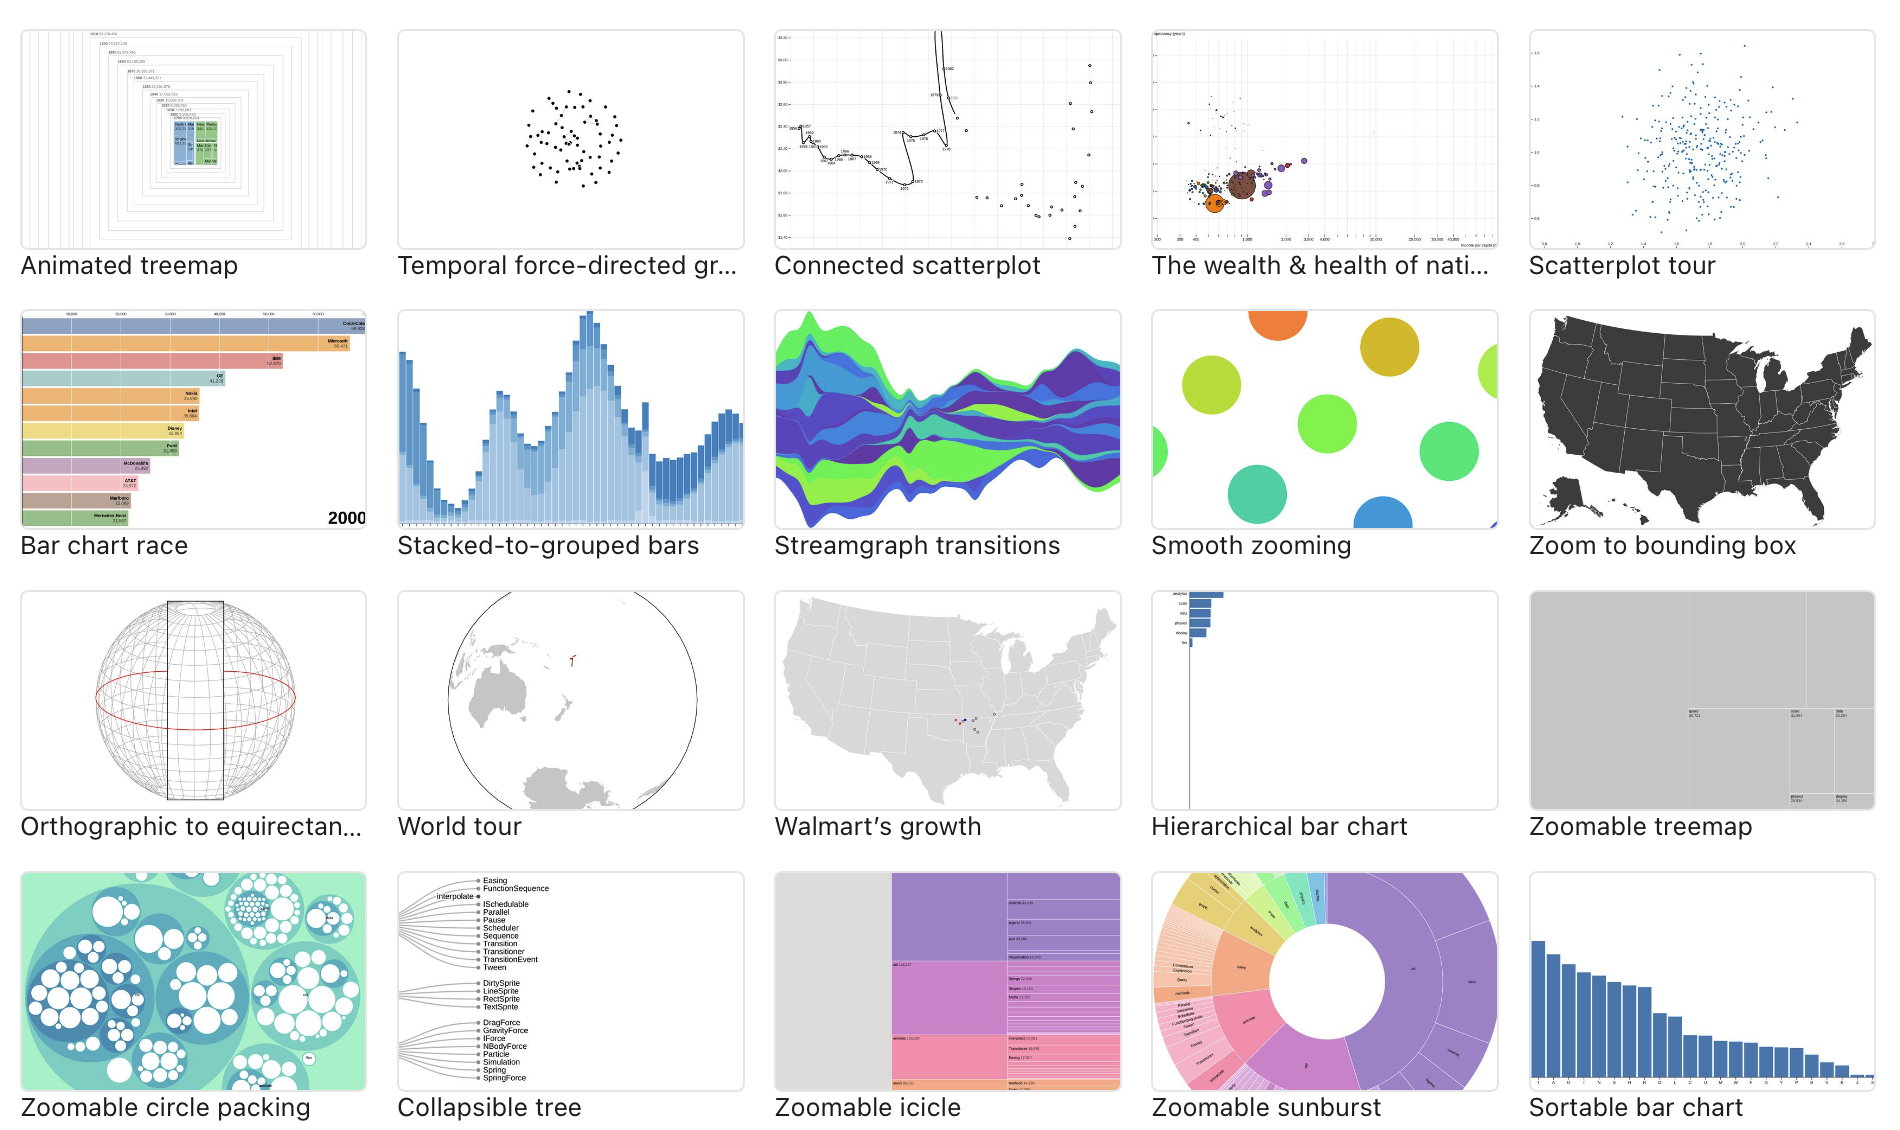
\includegraphics[width=0.9\textwidth]{Report-latex/tex_files/pics/d3.png}
\caption{Some D3 visualisations examples from D3 official website}
\end{figure}

\\\

\begin{figure}[H]
\centering
\captionsetup{justification=centering}
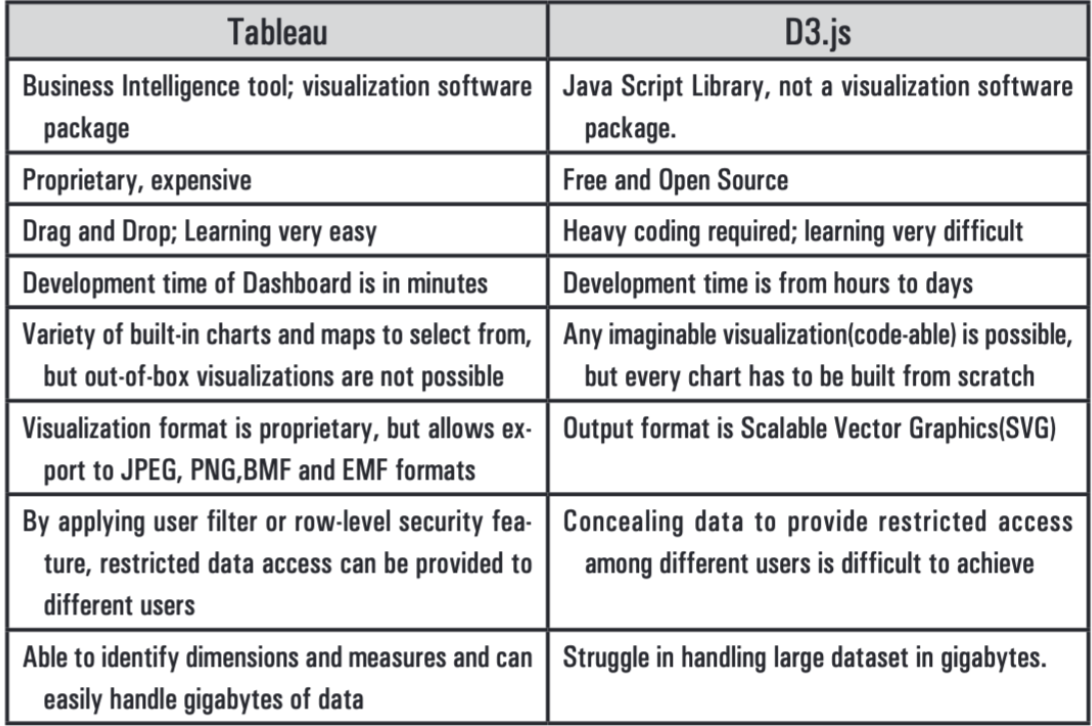
\includegraphics[width=0.7\textwidth]{Report-latex/tex_files/pics/tVd3.png}
\caption{Tableau vs D3 \cite{nair2016interactive}}
\end{figure}

\subsection{Dygraphs}



\subsection{Canvas}
Canvas.js is a javascript charting library with a simple API design and comes with a bunch of eye-catching themes. It is a lot faster than the conventional SVG or Flash charts. It also comes with a responsive design so that it can run on various devices like Android, iPhone, Tablets, Windows, Mac, etc.
The chart gallery consists of 24 different types of charts but the USP is its speed. It can render 100000 data points in just 100 milliseconds. Therefore, if you are looking for a high-performance javascript chart, Canvas can be your best bet. It boasts of some business giants like Intel, Apple, Boeing, and EMC2  in its clientele. However, this tool is free for non-commercial usage.


\subsection{Qlikview}
Qlik is one of the major players in the data analytics space with their Qlikview tool which is also one of the biggest competitors of Tableau.


\subsection{Microsoft Power BI}





\subsection{Infogram}
\subsection{ChartBlocks}
\subsection{Datawrapper}
\subsection{Plotly}

\subsection{Ember Charts}
uses d3

\subsection{NVD3}
runs on top of d3
\subsection{Google charts}
\subsection{Chart.js}
\subsection{Leaflet}
\subsection{Chartist.js}
\subsection{Sigma js}
\subsection{Fusion Chart}

